\scanpage{112}
\diagram{$\begin{array}{c|c}
\begin{gathered}
\mu_n\qquad\deleted{\unsure{(n,p)\neq1}}\ (n,p)=1\\
\begin{tikzcd}[row sep=small]\phantom{\mu_n}\arrow[d,squiggly]\\
\left[\operatorname{Grbg}(G_m)\xrightarrow{n}\operatorname{Grbg}(G_m)\right]\end{tikzcd}\\
[\,0\qquad1\,]\\
\figure{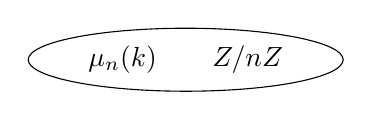
\begin{tikzpicture}\draw (0,0) ellipse (2 and .4);\node at(0,0){$\mu_n(k)\qquad\mathbb Z/n\mathbb Z$};\end{tikzpicture}}
\end{gathered}
&\begin{gathered}
\mathbb Z/n\mathbb Z\qquad(n,p)=1\\
\begin{tikzcd}[row sep=small]\phantom{\mathbb Z/n\mathbb Z}\arrow[d,squiggly]\\
\deleted{\mathbb Q/\mathbb Z\xrightarrow{n}\mathbb Q/\mathbb Z}\end{tikzcd}\\
0\qquad1\\
\figure{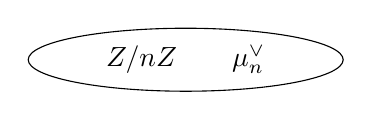
\begin{tikzpicture}\draw (0,0) ellipse (2 and .4);\node at(0,0){$\mathbb Z/n\mathbb Z\qquad\mu_n^\vee$};\end{tikzpicture}}
\end{gathered}\\\hline
\begin{gathered}
\begin{tikzcd}[row sep=small]\mu_p\arrow[d,squiggly]\\
\operatorname{Grbg}(G_m)\arrow[r,"p"]&\operatorname{Grbg}(G_m)\end{tikzcd}\\
[\,0\qquad1\,]\\
\figure{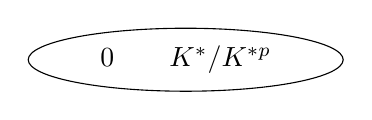
\begin{tikzpicture}\draw (0,0) ellipse (2 and .4);\node at(0,0){$0\qquad K^*/K^{*p}$};\end{tikzpicture}}
\end{gathered}
&\begin{gathered}
\begin{tikzcd}[row sep=small]\mathbb Z/p\mathbb Z\arrow[d,squiggly]\\
\operatorname{Grbg}(G_a)\arrow[r,"\wp"]&\operatorname{Grbg}(G_a)\end{tikzcd}\\
\figure{\begin{tikzpicture}\draw (0,0) ellipse (3.4 and .55);\node at(0,0){$\mathbb Z/p\mathbb Z\quad\underbrace{H^1(K,\mathbb Z/p\mathbb Z)}_{\substack{\text{cf corps de}\\\text{classe local}}}=\unsure{K^+/\wp K^+}$};\end{tikzpicture}}\\
\operatorname{Ext}^{0}(\unsure{K^*/K^{*p}},\mathbb Q/\mathbb Z)\qquad
\operatorname{Ext}_{\unsure{i}}(\unsure{K^*/K^{*p}},\mathbb Q/\mathbb Z)
\end{gathered}\\\hline
\begin{gathered}
\begin{tikzcd}[row sep=small]\alpha_p\arrow[d,squiggly]\\
\operatorname{Grbg}(G_a)\arrow[r,"\text{Frob}"]&\operatorname{Grbg}(G_a)\end{tikzcd}\\
\figure{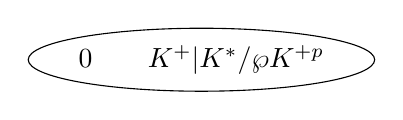
\begin{tikzpicture}\draw (0,0) ellipse (2.2 and .4);\node at(0,0){$0\qquad\unsure{K^+|K^*}/\deleted{\unsure{\wp}}K^{+p}$};\end{tikzpicture}}
\end{gathered}
&\begin{gathered}
\begin{tikzcd}[row sep=small]\alpha_p\arrow[d,squiggly]\\\unsure{\varsigma}\end{tikzcd}\\
\figure{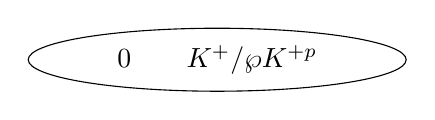
\begin{tikzpicture}\draw (0,0) ellipse (2.4 and .4);\node at(0,0){$0\qquad K^+/\deleted{\unsure{\wp}}K^{+p}$};\end{tikzpicture}}\qquad-
\end{gathered}\\\hline
\begin{gathered}
G_m\\
??\quad\figure{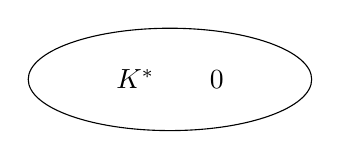
\begin{tikzpicture}\draw (0,0) ellipse (1.8 and .65);\node at(0,0){$K^*\qquad0$};\end{tikzpicture}}\\
\mathbb Z
\end{gathered}
&\begin{gathered}
\mathbb Z\qquad??\\
\figure{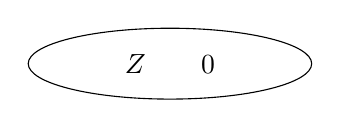
\begin{tikzpicture}\draw (0,0) ellipse (1.8 and .45);\node at(0,0){$\mathbb Z\qquad0$};\end{tikzpicture}}
\quad+H^1(K,\mathbb Q/\mathbb Z)
\end{gathered}
\end{array}$}
\figure{
\begin{tikzpicture}[x=.5cm,y=.3cm]
\draw (0,0)..controls(1,.7)and(1,-.5)..(2,0)..controls(3,.7)and(3,-.4)..(4,0)
..controls(5,.4)and(5,-.3)..(6,0)..controls(7,.5)and(7,-.4)..(8,0)
..controls(9,.7)and(9,-.4)..(10,0)..controls(11,.5)and(11,-.2)..(12,0);
\end{tikzpicture}}
\mspage{111}

